\documentclass[tikz,border=4mm]{standalone}
\usetikzlibrary{positioning,arrows.meta,intersections}
\usepackage{tikz}
\begin{document}
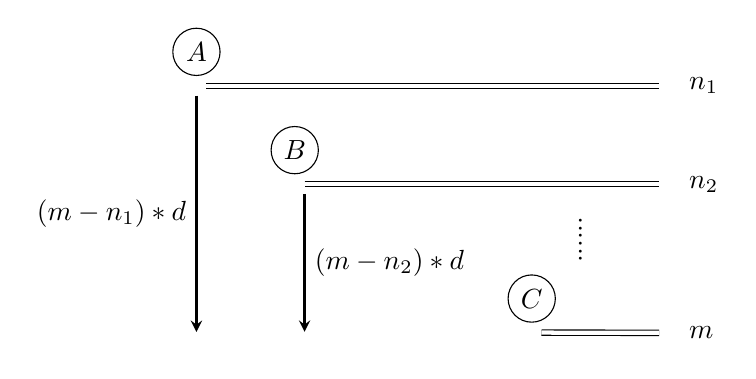
\begin{tikzpicture}[
    lev_num/.style={
        draw,circle, inner sep=0pt,minimum size=.6cm,node distance =.01mm,
    },
    double_lines/.style={
        double equal sign distance
    },
    arrow/.style={
        ->,thick,>={stealth[round]},
    }
]
    \node at (0, 0) (m1) {};
    \node at (6, 0) (m2) {};
    \node[lev_num,above= of m1](m3){$A$};
    \node[right=.01 of m2](){$n_1$};

    \node [below right=of m1](n1){};
    \node [below =of m2](n2){};
    \node [lev_num,above= of n1](){$B$};
    \node[right=.01 of n2](){$n_2$};

    \node[below left=of n2,right,rotate=90](p){$......$};

    \node[below left=0.9 of p](a1){};
    \node[below =1.64 of n2](a2){};
    \node [lev_num,above= of a1](){$C$};
    \node[right=.01 of a2](){$m$};

    \draw [double_lines](m1) to (m2);
    \draw [double_lines](n1) to (n2);
    \draw [double_lines](a1) to (a2);

    \node [below =3 of m1](m3){};
    \draw [arrow](m1.south) to node[midway,left]{$(m-n_1)*d$}(m3.north);

    \node [below =1.75 of n1](n3){};
    \draw [arrow](n1.south east) to node[midway,right]{$(m-n_2)*d$}(n3.north east);

    \end{tikzpicture}
\end{document}
